% arara: pdflatex: { shell: yes, interaction: nonstopmode }
% arara: pythontex: {verbose: yes, rerun: modified }
% arara: pdflatex: { shell: yes, interaction: nonstopmode }
% arara: clean: { extensions: [ aux, blg, idx, ilg, ind, log, out, pytxcode, rel, toc ] }
% !arara: clean: { files: [ ans.tex, hint.tex] }

% arara: pdflatex
% arara: clean: { extensions: [ aux, blg, idx, ilg, ind, log, out, pytxcode, rel, toc ] }
% !arara: clean: { files: [ ans.tex, hint.tex] }


\documentclass[queueing-book-solution.tex]{subfiles}
%\externaldocument{queueing-book}

\opt{solutionfiles,check}{
\loadgeometry{tufte}
\Opensolutionfile{hint}
\Opensolutionfile{ans}
}

\begin{document}


\section{Applications of Level-crossing, Little's law and PASTA}
\label{sec:mnmn1}

In this section we apply the tools developed up to now to many different queueing situations.
As an example, we discuss in considerable detail how to plan the number of cashiers at a supermarket such that the queue length remains small.
To keep the analysis simple, we approximate the $M/M/c$ queue by an $M/M/1$ with a server that is $c$ times as fast. So we first address the quality of this approximation.

The exercises at then end require quite some  modeling skills.
Hence, they are quite hard, even thought the formulas are simple.


It should be clear from~\cref{sec:mm1} that the expressions for, e.g., $\E\L$ are quite a bit harder for the $M/M/c$ queue than for the $M/M/1$.
To avoid using this complexity, it is tempting to approximate the $M/M/c$ queue by an $M/M/1$ queue with a server that works $c$ times as fast.
%As we now have the formulas for the $M/M/c$ queue and the $M/M/1$ queue, we can use these to obtain some basic understanding of the difference.

Let us therefore consider a numerical example.
Suppose that we have an $M/M/3$ queue with $\lambda = 5$ per day and $\mu=2$ per day per server, and we compare it to an $M/M/1$ with the same arrival rate but with a service rate of $\mu = 3\cdot 2 = 6$.
\begin{marginfigure}
\begin{pycode}[ratio]
from math import factorial
import numpy as np
import matplotlib.pylab as plt
import tikzplotlib
from matplotlib import style
style.use('ggplot')


def EL(labda, mu, c):
    rho = labda / mu / c
    G = sum((c * rho) ** n / factorial(n) for n in range(c))
    G += (c * rho) ** c / ((1 - rho) * factorial(c))
    Q = (c * rho) ** c / (factorial(c) * G) * rho / (1 - rho) ** 2
    L = Q + labda/mu
    return L


mu, c = 2., 3

L, load = [], []

for labda in np.linspace(0.1, 5.8, 20):
    L.append(EL(labda, mu, c) / EL(labda, c * mu, 1))
    load.append(labda / mu / c)

# plt.title("$M/M/3$ vs $M/M/1$")
plt.plot(load, L, label=r"$L_3/L_1$")
plt.xlabel("$\\rho$")
plt.legend()
plot = tikzplotlib.get_tikz_code(axis_height='5cm',
                                 axis_width='6cm')
print(plot)
\end{pycode}
\caption{The ratio of $\E\L$ for the $M/M/3$ and $M/M/1$ queue.}
\label{fig:fast}
\end{marginfigure}

The figure at the right shows the ratio of $\E\L$ for both queues as a function of $\rho$.
Clearly, when $\rho$ is small, this ratio is about $3$.
This is reasonable, because the service time in the fast $M/M/1$ is 3 times as small as the service time in the $M/M/3$ queue, and when $\rho$ is small, $\E\J \approx \E S$ because $\E\Q \approx 0$.\sidenote{Use Little's law to convert this statement about sojourn times into a  statement in terms of $\E \L$.}
However, when $\rho$ is large, $\E\J \gg \E S$, but jobs in queue do not `see' the difference between $c$ slow servers or one fast server. Therefore, the ratio becomes 1 as $\rho\uparrow 1$.


\newthought{Let us now discuss the} example of cashier planning of a supermarket.
We keep the analysis simple, as otherwise we would need sophisticated queueing models and data assembly tools.
Note however that the present example contains all  necessary steps to solve realistic planning problems.


We start with the arrival process distribution.
It is reasonable to model it as a Poisson process, as there are many potential customers, each choosing with a small probability to go to the supermarket at a certain moment in time.
Thus, we only have to characterize the arrival rate.
Estimating this for a supermarket is easy because the cash registers track all customers payments.
With this we have the number of customers that left, hence arrived at, the shop.

It is common to aggregate this data in a \emph{demand profile} which shows the average number of customers arriving per hour.
\begin{marginfigure}
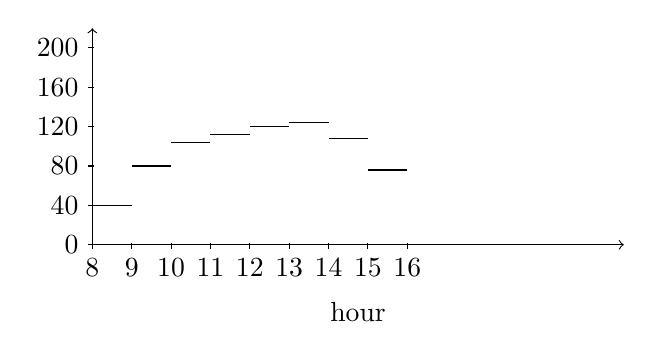
\begin{tikzpicture}[scale=.5]
    %axis
    \draw[->] (0,0) -- coordinate (x axis mid) (13.5,0);
    \draw[->] (0,0) -- coordinate (y axis mid) (0,5.5);
    %ticks
    \foreach \x in {0,...,8}
 \pgfmathsetmacro{\my}{int(\x+8)}
        \draw (\x,1pt) -- (\x,-3pt)
            node[anchor=north] {$\my$};
    \foreach \y in {0,...,5}
 \pgfmathsetmacro{\my}{int(\y*40)}
        \draw (1pt,\y) -- (-3pt,\y)
            node[anchor=east] {\my};
%labels
\node[below=0.6cm] at (x axis mid) {hour};
%\node[rotate=90, left=1.2cm] at (y axis mid) {$\lambda$};

\draw (0,1)--(1,1);
\draw (1,2)--(2,2);
\draw (2,2.6)--(3,2.6);
\draw (3,2.8)--(4,2.8);
\draw (4,3.)--(5,3.);
\draw (5,3.1)--(6,3.1);
\draw (6,2.7)--(7,2.7);
\draw (7,1.9)--(8,1.9);
% \draw (8,2.5)--(9,2.5);
% \draw (9,3.3)--(10,3.3);
% \draw (10,3.5)--(11,3.5);
%\draw (11,2.3)--(12,2.3);
%\draw (12,1.2)--(13,1.2);
\end{tikzpicture}
\caption{A demand profile.}
\label{fig:loadprofile}
\end{marginfigure}
Then we model the arrival process as Poisson with an arrival rate that is constant during a certain hour as specified by the demand profile.



It is also easy to find the service distribution from the cash registers.
The first item scanned after a payment determines the start of a new service, and the payment closes the service.\sidenote{As there is always a bit of time between the payment and the start of a new service we might add 15 seconds, say, to any service.}
To keep things simple here, we just model the service time distribution as exponential with mean $1.5$ minutes.

For the \emph{service objective} we consider the number of people in entire queueing system.
For ease, suppose there are 5 cashier positions, and that the queue per position should be at most 3.
Then there can be $5\cdot (1 + 3) = 20$ in the system before we say that the system is `too full'. As objective, let us set $\P{\L>20} < 1\%$.

Let us model the situation as an $M/M/1$ queue with a fast server, so that the objective becomes easy to compute.
In fact, since $\P{\L>n} = \rho^{n+1}$, we obtain the constraint $\rho\leq 0.8$.
In view of~\cref{fig:fast}, the difference in $\E \L$ between the multi-server and the single, but fast, server queue is small.


We now find a formula to convert the demand profile into a \emph{load profile} which specifies the minimal number of servers per hour needed to meet the service objective.
Using that $\rho = \lambda \E S/c \leq 0.8 $ and our estimate $\E{S}=1.5\cdot 60$ hour, we get the following rough bound on $c$:
\begin{equation*}
c \geq \lambda \frac{\E S}{0.8} \approx 0.03 \lambda.
\end{equation*}
For instance, for the hour from 12 to 13, we read in the demand profile~\cref{fig:loadprofile} that $\lambda= 120$ customers per hour, hence $c\approx 3.8 = 4$.

\newthought{The last step} is to \emph{cover the load profile with service shifts}.
This is typically not easy since shifts have to satisfy all kinds of rules.
For instance, a shift length must be at least four hours, and no longer than 9 hours including breaks.
Or, when the shift is longer than 4 hours it needs to contain at least one break of 30 minutes.
Shifts can also have different costs: evening shifts are typically  more expensive per hour.

The usual way to solve such covering problems is by means of an integer
problem. For instance, suppose only 4 \emph{shift plans} are available as shown at the right.\sidenote{\begin{enumerate}
\item $++-++$
\item $+++-+$
\item $++-+++$
\item $+++-++$,
\end{enumerate}
Shift plans. A $+$ indicates a working hour and $-$ a break of an hour.}
Then generate \emph{shift types} where a shift type is a shift plan that starts at a certain hour.

For the optimization, let $x_i$ be the number of shifts of type $i$ and~$c_i$ the cost of this type.
Then the problem is to solve $\min \sum_i c_i x_i$,
such that for all hours $t$ the shifts cover the load, i.e., $\sum_i x_i \1{t \in s_i} \geq 0.03 \lambda_t$.
(We write $t\in s_i$ if hour $t$ is covered by shift type $i$.)

\begin{exercise}[Hall 5.6]
  An $M/M/1$ queue has been found to have an average waiting time in queue of 1 minute.
  The arrival rate is known to be 5 customers per minute.
  What are the service rate and utilization?
  Calculate $\E{\Q}$, $\E \L$ and $\E\W$.
  Finally, the queue operator would like to provide chairs for waiting customers.
  He would like to have a sufficient number so that all (waiting and in service) customers can sit down at least 90 percent of the time.
  How many chairs should he provide?

\begin{hint}
  $\E{\Q}$ follows right away from an application of Little's law.
  For the other quantities we need to find $\E S$.
  Use the expression for  $\E{\W(M/M/1)}$ to solve for $\rho$. Then, since $\lambda$ is known, $\E S$ follows.
\end{hint}
\begin{solution} With Little's law:
\begin{pyconsole}
labda = 5. # per minute
W = 1.
Q = labda*W
Q
\end{pyconsole}

We can use the expression for $\E\W$ to solve for $\rho$, but we also do a simple search.
\begin{pyconsole}
from scipy.optimize import bisect


def find_W(rho): # return W -1 for given rho
    ES = rho / labda
    return rho / (1 - rho) * ES - 1


rho = bisect(find_W, 0, 0.999)
rho
ES = rho/labda
ES
J = W + ES
J
L = labda*J
L
\end{pyconsole}
Next, find $n$ such that $\sum_{j=0}^n p_j > 0.9$.
\begin{pyconsole}
n, total, p = 0, 0.0, 1 - rho
while total <= 0.9:
    total += p
    n += 1
    p *= rho

total
n
\end{pyconsole}
Note that we increased $n$ one time too often. As a check,  use that $(1-\rho) \sum_{j=0}^n \rho^j = 1-\rho^{n+1}$.
\begin{pyconsole}
n -= 1 # get the right n
1-rho**(n) # this must be too small.
1-rho**(n+1) # this must be OK.
\end{pyconsole}
\end{solution}
\end{exercise}


\begin{exercise}[Hall 5.3]\label{ex:l-823}

  After observing a queue with two servers for several days, the following steady-state probabilities have been determined: $p(0)=0.4$, $p(1) = 0.3$, $p(2)=0.2$, $p(3)=0.05$ and $p(4)=0.05$.
  The arrival rate is 10 customers per hour.
 Determine $\E \L$, $\E{\Q}$, $\E \J$, $\E{\W}$, $\V \L$ and $\V{\Q}$. Finally, compute the service time and the utilization.
\begin{solution}
Start with the data, then do the computations.
\begin{pyconsole}
c = 2
p = [0.4, 0.3, 0.2, 0.05, 0.05]
labda = 10.0 / 60 # per hour

EL = sum(n * p[n] for n in range(len(p)))
EL
EQ = sum(max(n - c, 0) * p[n] for n in range(len(p)))
EQ
W = EQ / labda  # in minutes
W
J = EL / labda  # in minutes
J
var_L = sum((n - EL) ** 2 * p[n] for n in range(len(p)))
var_L
var_Q = sum((max(n - c, 0) - EQ) ** 2 * p[n] for n in range(len(p)))
var_Q
ES = J - W
rho = labda * ES / c
rho
\end{pyconsole}

The expected number of busy servers is the average number in the system minus the average number in queue.
It should also be equal to $\sum_{n=0}^\infty \min\{n,c\} p(n)$.
Let's check.
\begin{pyconsole}
EBusy = EL - EQ
EBusy
u = sum(min(n, c) * p[n] for n in range(len(p)))
u
\end{pyconsole}
\end{solution}
\end{exercise}

\begin{exercise}
 (Hall 5.14) An airline phone reservation line has one server and a buffer for two customers.
 The arrival rate is 6 customers per hour, and a service rate of just 5 customers per hour.
 Arrivals are Poisson and service times are exponential.
 Estimate $\E{\Q}$ and the average number of customers served per hour.
 Then, estimate $\E{\Q}$ for a buffer of size~5.
 What is the impact of the increased buffer size on the number of customers served per hour?
\begin{hint}
This is an $M/M/1/3$ queue; there is room for 1 customer in service and two in queue.
\end{hint}
\begin{solution}
We import \pyv{numpy} and convert the lists to arrays is to fix the output precision to 3, otherwise we get long floats in the output.

First the case with $b=2$.
\begin{pyconsole}
import numpy as np
np.set_printoptions(precision=3)

labda, mu, c = 6.0,  5.0, 1
rho = labda / mu
K = c + 2


p = np.array([rho ** n for n in range(K + 1)]) # range(n) is up to n
G = sum(p)
p /= G  # normalize
p
L = sum(n * p[n] for n in range(len(p)))
L
Q = sum(max(n - c,0) * p[n] for n in range(len(p)))
Q
lost = labda * p[-1]  # the last element of p
labda - lost # accepted, hence served
\end{pyconsole}

Now increase the buffer $b$ to 5.

\begin{pyconsole}
K = c + 5
p = np.array([rho ** n for n in range(K + 1)]) # range(n) is up to n
G = sum(p)
p /= G  # normalize
lost = labda * p[-1]  # the last element of P
labda - lost # accepted, hence served
\end{pyconsole}
We see that since the server is overloaded, the acceptance is not much affected by increasing the buffer space.
We need an extra server.
\end{solution}
\end{exercise}


\begin{exercise}[Hall 5.8]\label{ex:39}
The queueing system at a fast-food stand behaves in a peculiar fashion.
 When there is no one in the queue, people are reluctant to use the stand, fearing that the food is unsavory.
 People are also reluctant to use the stand when the queue is long.
 This yields the following arrival rates (in numbers per hour): $\lambda(0) = 10$, $\lambda(1)=15$, $\lambda(2)=15$, $\lambda(3)=10$, $\lambda(4)=5$, $\lambda(n)=0, n\geq 5$.
 The stand has two servers, each of which can operate at 5 per hour.
 Service times are exponential, and the arrival process is Poisson.
 Calculate the steady state probabilities.
 Next, what is the average arrival rate?
 Finally, determine $\E \L$, $\E{\Q}$, $\E \J$ and $\E{\J}$.
\begin{hint}
This is a queue with balking.
\end{hint}
\begin{solution}
The computations.
\begin{pyblock}
import numpy as np

labda = np.array([10.0, 15.0, 15.0, 10.0, 5.0])
mu = np.array([0., 5., 10., 10., 10., 10.])
c = 2

p = np.ones_like(mu)
for i in range(len(labda)):
    p[i+1] = labda[i] *p[i]/ mu[i+1]

p /= p.sum()
labdaBar = sum(labda[n] * p[n] for n in range(len(labda)))
L = sum(n * p[n] for n in range(len(p)))
Q = sum(max(n - c,0) * p[n] for n in range(len(p)))
J = L / labdaBar
W = Q / labdaBar
\end{pyblock}

\end{solution}
\end{exercise}

\begin{exercise}[Hall 5.10]\label{ex:l-217}
A repair/maintenance facility would like to determine how many employees should be working in its tool crib.
\marginpar{Recall, in queueing systems always somebody has to wait, either a customer in queue or a server being idle.
If it is very expensive to let customers wait, the number of servers must be high, whereas if servers are relatively expensive, customers have to do the waiting.}
 The customers are actually maintenance workers at the facility, and are compensated at the same rate as the tool crib employees.
 The service time is exponential, with mean 4 minutes, and customers arrive by a Poisson process with rate 28 per hour.
 What is $\E \W$ for $c=1, 2, 3$, or $4$ servers?
 How many employees should work in the tool crib?
\begin{hint}
We are dealing with an $M/M/c$ queue. And, what is the implication of the remark about the compensation rate?
\end{hint}
\begin{solution}
What is the load?
\begin{pyconsole}
labda = 28.0 / 60  # arrivals per minute
ES = 4.0
labda * ES
\end{pyconsole}
Clearly, we need at least two servers.

\begin{pyconsole}
from math import factorial


def Q(labda, ES, c):
    rho = labda * ES / c
    G = sum([(c * rho) ** n / factorial(n) for n in range(c)])
    G += (c * rho) ** c / (1.0 - rho) / factorial(c)
    return (c * rho) ** c / (factorial(c) * G) * rho / (1.0 - rho) ** 2

Q(labda, ES, c=2)/labda  # in minutes, Little's law
Q(labda, ES, c=3)/labda  # in minutes, Little's law
Q(labda, ES, c=4)/labda  # in minutes, Little's law
\end{pyconsole}


Since both types of workers cost the same amount of money per unit time, it is best to divide the amount of waiting/idleness equally over both types of workers.
The average cost of workers waiting in queue is proportional to $\E \Q$.  At the crib, the load is $\lambda \E S$, hence, the average number of idle server is $c-\lambda \E S$.

\begin{pyconsole}
c = 2
Q(labda, ES, c) + (c - labda * ES)
c = 3
Q(labda, ES, c) + (c - labda * ES)
c = 4
Q(labda, ES, c) + (c - labda * ES)

\end{pyconsole}
\end{solution}
\end{exercise}

\begin{exercise}[Hall 5.22]\label{ex:95}
 At \marginpar{This is a bit hard, but important problem; it is the same as an inventory system with backlogging in which taxis act as products on hand and parties as customers.} a large hotel, taxi cabs arrive at a rate of 15 per hour, and parties of riders arrive at the rate of 12 per hour.
 Whenever taxicabs are waiting, riders are served immediately upon arrival.
 Whenever riders are waiting, taxicabs are loaded immediately upon arrival.
 A maximum of three cabs can wait at a time (other cabs must go elsewhere).
First find an appropriate way to model this queueing system as an $M/M/1$ queue. Then
 calculate the expected number of cabs waiting and the expected number of parties waiting, and the average waiting times of cabs and parties.
 What would be the impact of allowing four cabs to wait at a time?
Assume that all members of a party of riders can be served by a single cab, that is, the parties do not exceed the capacity of a cab and all members of a party have the same destination.
\begin{hint}
  Let $p_{ij}$ be the fraction of time that the system contains $i$ riders and $j$ taxi cabs.
  When a group arrives, they take a taxi, so the number of taxis decreases by one. If there are no taxis, the group has to wait.
  When a new taxi arrives, the number of groups is reduced by one, and so on, until there are $3$ taxis waiting and no groups of people.
Thus group arrivals acts as job arrivals, and taxi arrivals as services.
Here is an overview of the transitions  where  $\mu$ is the rate at which cabs arrive, and $\lambda$ is the arrival rate of parties of riders.
 \begin{center}
\begin{tikzpicture}[->,>=stealth',shorten >=1pt,auto,node distance=1.8cm,
 semithick]
 \node[state] (0) {$p(0,3)$} ;
 \node[state] (1) [right of=0] {$p(0,2)$};
 \node[state] (2) [right of=1] {$p(0,1)$};
 \node[state] (3) [right of=2] {$p(0,0)$};
 \node[state] (4) [right of=3] {$p(1,0)$};
 \node[state] (5) [right of=4] {$p(2,0)$};
 \node[state] (6) [right of=5] {$p(\cdot, 0)$};

\path
 (0) edge [bend left] node {$\lambda$} (1)
 (1) edge [bend left] node {$\mu$} (0)
 (1) edge [bend left] node {$\lambda$} (2)
 (2) edge [bend left] node {$\mu$} (1)
 (2) edge [bend left] node {$\lambda$} (3)
 (3) edge [bend left] node {$\mu$} (2)
 (3) edge [bend left] node {$\lambda$} (4)
 (4) edge [bend left] node {$\mu$} (3)
 (4) edge [bend left] node {$\lambda$} (5)
 (5) edge [bend left] node {$\mu$} (4)
 (5) edge [bend left] node {$\lambda$} (6)
 (6) edge [bend left] node {$\mu$} (5)
;
\end{tikzpicture}
 \end{center}
Now map this system to an $M/M/1$ queue.
\end{hint}
\begin{solution}
  From the figure in the hint, the situation with the taxis corresponds to an $M/M/1$ queue, only the states have a `different name'.
  Let $l$ be the number of jobs in an M/M/1 queue.
  To make a mapping from $l$ to the number of parties $i$ and number of taxis $j$, observe that $l = 3 - j +i$ and $\1{j>0}\1{i>0} = 0$, because riders don't wait when there are taxis available. To see this,  consider the following table
\begin{center}
\begin{tabular}{ccc}
$j$ & $i$ & $l$\\
3& 0 & 0\\
2 & 0& 1\\
1 & 0& 2\\
0& 0& 3\\
0& 1& 4\\
0& 2& 5\\
\end{tabular}
\end{center}

With this mapping, the expected number of taxis $T$ is $\E T =  \sum_{l=0}^3 (3-l)p(l)$.
\begin{pyconsole}
labda = 12.0  # per hour
mu = 15.0  # per hour
rho = labda / mu
n = 3  # number of taxis

ET, p = 0, 1 - rho
for l in range(n):
    ET += (n - l) * p
    p *= rho

ET
\end{pyconsole}
For the expected number of groups waiting note that $l=3-j+i$ always.
Taking expectations, we see that $\E \L = 3 - \E T + \E G$, where $\E G$ is the expected number of groups.
\begin{pyconsole}
EL = rho/(1-rho)
EG = EL-n + ET
EG
\end{pyconsole}

Computing the waiting times is tricky. For the taxis, the rate at which `jobs' arrive, is the arrival rate of the riders. For the riders, the rate at which `jobs' arrive is the arrival rate of taxis.
\begin{pyconsole}
ET/labda # Waiting for taxis
EG/mu # waiting time for groups
\end{pyconsole}

What would be the impact of allowing 4 cabs?
\begin{pyconsole}
n = 4  # number of taxis

ET, p = 0, 1 - rho
for l in range(n):
    ET += (n - l) * p
    p *= rho

ET
EG = EL-n + ET
EG
\end{pyconsole}
\end{solution}
\end{exercise}


\begin{exercise}
Suppose\marginpar{Continuation of~\cref{ex:95}} cabs are not allowed to wait. What is the expected waiting time for a party of riders?

\begin{solution}
This is a case with $n=0$, hence $\E G = \E \L$.
\end{solution}
\end{exercise}

\begin{exercise}\label{ex:l-219}
 Suppose\marginpar{Continuation of~\cref{ex:95}.
This one is quite  hard.}
cabs can contain at most 4 riders, and the size of a party (i.e., a batch) has distribution $B_k$ with $\P{B_k= i} = 1/7$ for $i=1,\ldots, 7$.
Parties of riders have the same destination, so riders of different parties cannot be served by one taxi.
Provide a set of recursions to simulate this system.

\begin{solution}
 We concentrate on departure epochs of the taxis.
 Thus, the $k$th period is the time between the departure of taxi $k-1$ and taxi $k$.
 During the $k$th epoch $a_k$ batches can arrive.
 The system starts with $a_0$ batches in queue.


 More generally, consider the arrival of taxi $k$. Let this taxi see $\Q_{s,k}$  riders at the head of the line. Let $b$ be the index of the first group in the queue, hence group $b-1$ stands at the head of the line. Then,
\begin{align*}
d_k &= \min\{\Q_{s,k}, 4\}, &\text{riders served by taxi $k$}, \\
\Q_{s}' &= \Q_{s,k} - d_k, &\text{riders remaining behind at head of line}, \\
\Q_k' &= \Q_k + a_{k+1}, &\text{groups just before arrival taxi $k+1$}, \\
h_k &= \1{\Q_s'>0}\1{\Q_k'>0} & \text{If $h_k=1$ a group can move to the head of the line}, \\
\Q_{k+1} &= \Q_k' - h_k& \text{queue of groups seen by taxi $k+1$}, \\
\Q_{s, k+1} &= \Q_{s}'(1-h_k) + h_k B_b& \text{riders at head of the line seen by taxi $k+1$}, \\
b &= b + h_k & \text{increase index of served batches by one}, \\
\end{align*}

\end{solution}

\end{exercise}


\opt{solutionfiles}{\Closesolutionfile{hint}
\Closesolutionfile{ans}
\loadgeometry{normal}
\input{hint}
\input{ans}
}

\end{document}





%%% Local Variables:
%%% mode: latex
%%% TeX-master: t
%%% End:
